% Templates
\begin{comment}

\begin{figure}[H]
	\centering
	\includegraphics[width=0.7\textwidth]{operasjonsforsterker/}
	\caption{}
	\label{fig:}
\end{figure}

\vspace{0.5cm} % Add space after the solution

\begin{enumerate}[label=\roman*)]
	\item
	\item
\end{enumerate}

\begin{question}[name=Oppgave, topic=operasjonsforsterker]

	\begin{enumerate}[label=\roman*)]
		\item
		\item
		\item
	\end{enumerate}
\end{question}

\vspace{0.5cm} % Add space after the solution

\begin{solution}[name=Løsningsforslag oppgave]
	Symboler vist i Figur \ref{fig:}.
	\begin{figure}[H]
		\centering
		\includegraphics[width=0.7\textwidth]{}
		\caption{}
		\label{fig:}
	\end{figure}
\end{solution}
\end{comment}

%--------------------------- GENERELT --------------------------------
\begin{question}[name=Oppgave, topic=operasjonsforsterker]
	En integrert operasjonsforsterker har
	\begin{enumerate}[label=\roman*)]
		\item To innganger og to utganger
		\item Én inngang og én utgang
		\item To innganger og én utganga
	\end{enumerate}
\end{question}

\begin{solution}[name=Løsningsforslag oppgave]
	Riktig svar: iii

\end{solution}
\vspace{0.5cm} % Add space after the solution
\begin{question}[name=Oppgave, topic=operasjonsforsterker]
	Hvilken av disse egenskapene beskriver en operasjonsforsterker dårligst
	\begin{enumerate}[label=\roman*)]
		\item Høy forsterkning
		\item Høy inngangsmotstand
		\item Lav effekt
		\item Lav utgangsresistans
	\end{enumerate}
\end{question}

\begin{solution}[name=Løsningsforslag oppgave]
	Riktig svar: iii

\end{solution}
\vspace{0.5cm} % Add space after the solution
\begin{question}[name=Oppgave, topic=operasjonsforsterker]
	Med $0[V]$ på begge inngangene skal en ideell operasjonsforsterker ha hva på utgangen
	\begin{enumerate}[label=\roman*)]
		\item Positiv driftspenning $+V_{cc}$
		\item Negativ driftspenning $-V_{cc}$
		\item $0[V]$
	\end{enumerate}
\end{question}

\begin{solution}[name=Løsningsforslag oppgave]
	Riktig svar: iii

\end{solution}
\vspace{0.5cm} % Add space after the solution
\begin{question}[name=Oppgave, topic=operasjonsforsterker]
	Av verdiene nevnt i listen, hvilken at de beskriver den mest realistiske verdien for operasjonforsterkerens forsterkning uten tilbakekobling.
	\begin{enumerate}[label=\roman*)]
		\item 1
		\item 2000
		\item 80[dB]
		\item 100000
	\end{enumerate}
\end{question}

\begin{solution}[name=Løsningsforslag oppgave]
	Riktig svar: iv
\end{solution}
\vspace{0.5cm} % Add space after the solution

\begin{question}[name=Oppgave, topic=operasjonsforsterker]
	Velg det riktige alternativet for egenskapene til en ideell operasjonsforsterker.

	\begin{enumerate}[label=\roman*)]
		\item Hvilke tilkoblinger har en standard operasjonsforsterker?
		\item Hvordan er spenningsforsterkning for en ideell operasjonsforsterker annerledes enn for en fysisk operasjonsforsterker?
		\item Hva indikerer $+$ tegnet på den ene inngangen av operasjonsforsterkeren?
		\item
	\end{enumerate}
\end{question}

\vspace{0.5cm} % Add space after the solution

\begin{solution}[name=Løsningsforslag oppgave]

	\begin{enumerate}[label=\roman*)]
		\item Inverterende og ikke-inverterende innganger, utgang, positiv og negativ tilførsel
		\item En fysisk operasjons-forsterker har stor spenningsforsterkning, men ikke uendelig som vi antar for den ideelle modellen
		\item Ikke-inverterende inngang
	\end{enumerate}

\end{solution}

\vspace{0.5cm} % Add space after the solution
\begin{question}[name=Oppgave, topic=operasjonsforsterker]
Velg det riktige alternativet for egenskapene til en ideell operasjonsforsterker.

	\begin{enumerate}[label=\roman*)]
	\item Inngangsimpedans = 0 og utgangsimpedans = 0
	\item Inngangsimpedans = 0 og utgangsimpedans = $\infty$
	\item Inngangsimpedans = $\infty$ og utgangsimpedans = 0
	\item Inngangsimpedans = $\infty$ og utgangsimpedans = $\infty$
\end{enumerate}
\end{question}

\vspace{0.5cm} % Add space after the solution

\begin{solution}[name=Løsningsforslag oppgave]
	Riktig svar er iii.

\end{solution}
\vspace{0.5cm} % Add space after the solution


\begin{question}[name=Oppgave, topic=operasjonsforsterker]
Ta utgangspunkt i delenummer TL081P og det vedlagte databladet presentert i Vedlegg \ref{paper-b} for å svare på følgende:
	\begin{enumerate}[label=\roman*)]
	\item Tegn opp en prinsippskisse for hvordan man kan koble opp en inverterende og ikke-inverterende kobling
	\item Hva er den maksimale spenningen brikken kan drives med, og hva er den maksimale spenningen den bør drives med.
	\item Hva er den maksimale spenningen man kan ha inn på inngangen
	\end{enumerate}



\end{question}

\vspace{0.5cm} % Add space after the solution

\begin{solution}[name=Løsningsforslag oppgave]


\end{solution}
\vspace{0.5cm} % Add space after the solution


\begin{question}[name=Oppgave, topic=operasjonsforsterker]
Studer kretsene vist i Figur \ref{fig:basicOpamp1}, Figur \ref{fig:basicOpamp2} og Figur \ref{fig:basicOpamp3} forså å angi hva utgangspenningen er for de forskjellige koblingene.

	\begin{figure}[H]
		\centering
		\begin{minipage}{0.45\textwidth}
			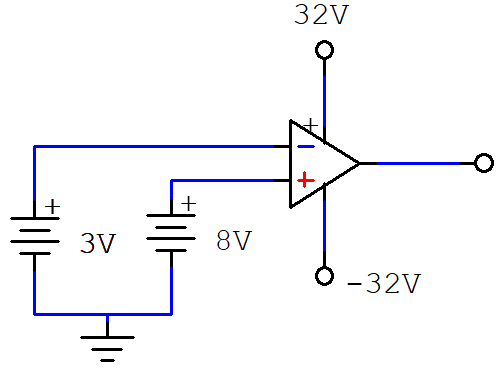
\includegraphics[width=\textwidth]{operasjonsforsterker/figurer/basic1.png}
			\caption{Kobling 1}
			\label{fig:basicOpamp1}
		\end{minipage}\hfill
		\begin{minipage}{0.45\textwidth}
			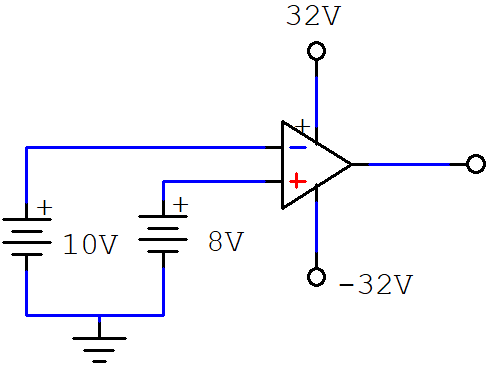
\includegraphics[width=\textwidth]{operasjonsforsterker/figurer/basic2.png}
			\caption{Kobling 2}
			\label{fig:basicOpamp2}
		\end{minipage}\par
		\vskip\floatsep% normal separation between figures
		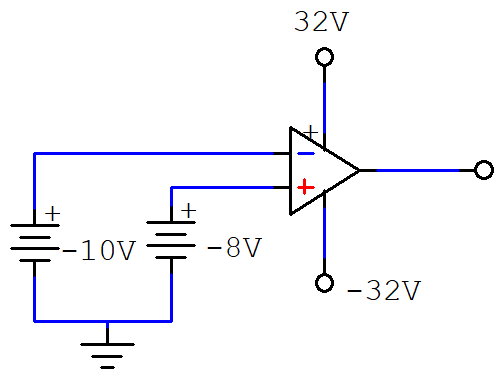
\includegraphics[width=0.45\textwidth]{operasjonsforsterker/figurer/basic3.png}
		\caption{Kobling 3}
		\label{fig:basicOpamp3}
	\end{figure}

\end{question}

\vspace{0.5cm} % Add space after the solution

\begin{solution}[name=Løsningsforslag oppgave]
Kobling 1: $U_{ut}=32[V]$

Potensialet på den ikke-inverterende inngangen er høyere enn potensialet på den inverterende. Utgangen vil derfor gå til maksimum positiv spenning bare begrenset av driftspenningen til kretsen.

Kobling 2: $U_{ut}=-32[V]$

Potensialet på den inverterende inngangen er høyere enn potensialet på den ikke-inverterende. Utgangen vil derfor gå til maksimum negativ spenning bare begrenset av driftspenningen til kretsen.

Kobling 3: $U_{ut}=32[V]$

Potensialet på den inverterende inngangen er høyere enn potensialet på den ikke-inverterende ved at spenningen på den ikke-inverterende er mindre negativt enn potensialet på den inverterende. Utgangen vil derfor gå til maksimum positiv spenning bare begrenset av driftspenningen til kretsen.

\end{solution}
\vspace{0.5cm} % Add space after the solution

%--------------------------- INVERTERNENDE KOBLING --------------------------------
\begin{question}[name=Oppgave, topic=operasjonsforsterker]
En operasjonsforsterkerkrets er koblet som inverterende forsterker. Kretsens forsterkning $F_U = -200$ med en inngangsresistans / serieresistans angitt til $R_1=10[k\Omega]$.

	\begin{enumerate}[label=\roman*)]
		\item Beregn motstandsverdien for $R_2$.
		\item Hva er spenningen man måler man på utgangen av koblingen, dersom inngangspenningen er $1[V_{DC}]$
	\end{enumerate}


\end{question}

\vspace{0.5cm} % Add space after the solution

\begin{solution}[name=Løsningsforslag oppgave]

		\begin{enumerate}[label=\roman*)]
		\item
\[F_U =- \frac{R_K}{R_1} \rightarrow -200= \frac{R_K}{10 \cdot 10^3} \rightarrow -200 \cdot 10 \cdot 10^3 = -R_K \rightarrow R_K = 200 \cdot 10 \cdot 10^3 = 2[M\Omega]\]

		\item
\[U_{ut}=-\frac{R_K}{R_{inn}} \cdot U_{inn} = -\frac{2\cdot 10^6}{10 \cdot 10^3} \cdot 1 = -200[V]\]

Operasjonsforsterkerens utgangspenning blir begrense av $\pm V_{CC}$.
	\end{enumerate}

\end{solution}
\vspace{0.5cm} % Add space after the solution

\begin{question}[name=Oppgave, topic=operasjonsforsterker]
		\begin{enumerate}[label=\roman*)]
			\item Kretsen som vist i Figur \ref{fig:invKobling} er koblet slik at forsterkningen $F_U = 2$. Kretsen blir påtrykt et signal som vist i Figur \ref{fig:invPlot}. Tegn utgangsignalet sammen med inngangsignalet for kretsen.

			\item Si noe om hvordan forholdet mellom $R_1$ og $R_2$ må være for at kretsen skal ha $F_U = 2$. Foreslå motstandsverdier for $R_1$ og $R_2$.
		\end{enumerate}
	\begin{figure}[H]
	\begin{minipage}[c]{0.45\linewidth}
		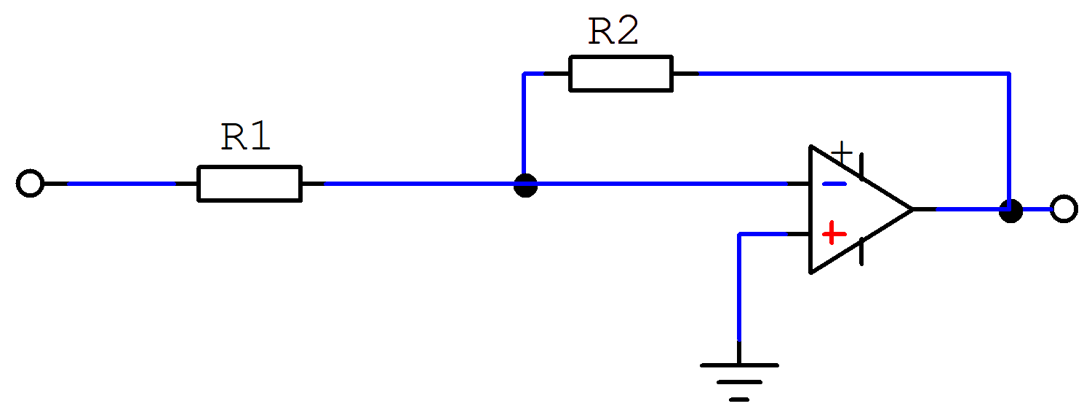
\includegraphics[width=\linewidth]{operasjonsforsterker/figurer/invBasic.png}
		\caption{Krets med operasjonforsterker}
		\label{fig:invKobling}
	\end{minipage}
	\hfill
	\begin{minipage}[c]{0.45\linewidth}
		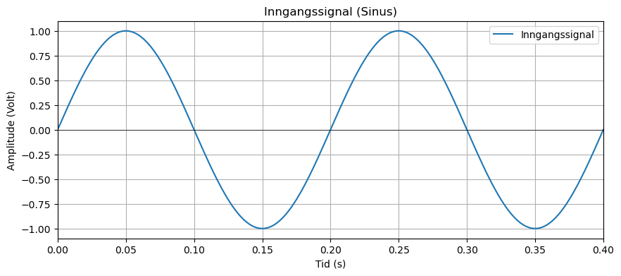
\includegraphics[width=\linewidth]{operasjonsforsterker/plot/InvPlot.png}
		\caption{Inngangsignal til krets}
		\label{fig:invPlot}
	\end{minipage}
\end{figure}

\end{question}

\vspace{0.5cm} % Add space after the solution

\begin{solution}[name=Løsningsforslag oppgave]
		\begin{enumerate}[label=\roman*)]
	\item
		\begin{figure}[H]
		\centering
		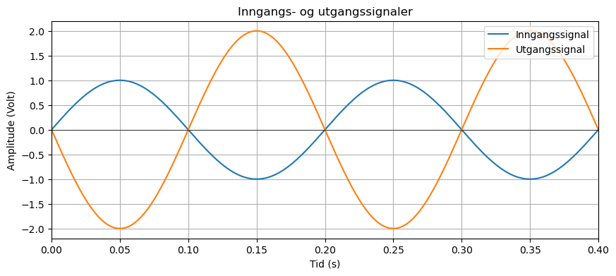
\includegraphics[width=0.7\textwidth]{operasjonsforsterker/plot/InvPlotSOL.png}
		\caption{Inngang og utgangsignal for en inverterende kobling}
		\label{fig:invPlotSOL}
	\end{figure}
	\item Den generelle spenningsforsterkningen for en inverterende kobling kan beskrives ved formelen som vist i Formel \ref{eqn:opAmpForsterk}.

	\begin{equation}
		\label{eqn:opAmpForsterk}
		F_U = -\frac{R_K}{R_{inn}}
	\end{equation}

Dersom man ønsker er forsterkning $F_U=-1$ vil det si at $R_K$ og $R_{inn}$ må ha samme verdi slik at når de deles på hverandre blir resultatet 1. Dersom man ønsker en dobling av forsterkningen må tallet i teller være dobbelt så stort som i nevner for at resultatet skal bli 2. Et eksempel:

\[F_U=-\frac{2}{1}=2\]

Så ved en teoretisk betraktning kan man derfor si at forholdet mellom motstandene sier noe om forsterkningen, og ikke verdien på motstandene. Derfor kan alternative verdier være $R_K=2 [\Omega]$ og $R_{inn}=1[\Omega]$, eller $R_K=2 [M\Omega]$ og $R_{inn}=1[M\Omega]$

\end{enumerate}
\end{solution}
\vspace{0.5cm} % Add space after the solution


\begin{question}[name=Oppgave, topic=operasjonsforsterker]
Finn verdien for $R_2$ i for kretsen vist i Figur \ref{fig:invCircuit1} slik at $F_U=100$.
\begin{figure}[H]
	\centering
	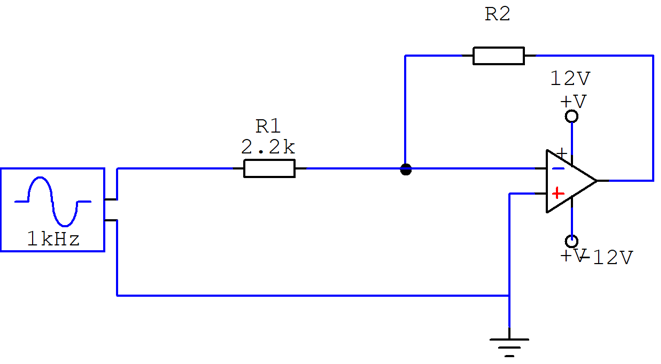
\includegraphics[width=0.7\textwidth]{operasjonsforsterker/figurer/invBasicCir.png}
	\caption{Operasjonsforsterkerkrets}
	\label{fig:invCircuit1}
\end{figure}

\end{question}

\vspace{0.5cm} % Add space after the solution

\begin{solution}[name=Løsningsforslag oppgave]

\[F_U = -\frac{R_2}{R_1} \rightarrow -100 = -\frac{R_2}{2,2 \cdot 10^{3}} \rightarrow (-100) \cdot 2,2 \cdot 10^3 = -R_2 \cdot 1 \rightarrow R_2 = 220 [k\Omega]\]

\end{solution}
\vspace{0.5cm} % Add space after the solution


%--------------------------- IKKE INVERTERNENDE KOBLING --------------------------------


\begin{question}[name=Oppgave, topic=operasjonsforsterker]

Kretsen som vist i Figur \ref{fig:NONinvKobling} er koblet slik at forsterkningen $F_U = 2$. Kretsen blir påtrykt et signal som vist i Figur \ref{fig:NONinvPlot}. Tegn utgangsignalet sammen med inngangsignalet for kretsen.

	\begin{figure}[H]
		\begin{minipage}[c]{0.45\linewidth}
			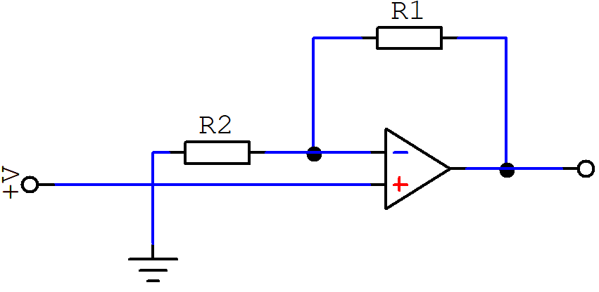
\includegraphics[width=\linewidth]{operasjonsforsterker/figurer/NONinvBasic.png}
			\caption{Krets med operasjonforsterker}
			\label{fig:NONinvKobling}
		\end{minipage}
		\hfill
		\begin{minipage}[c]{0.45\linewidth}
			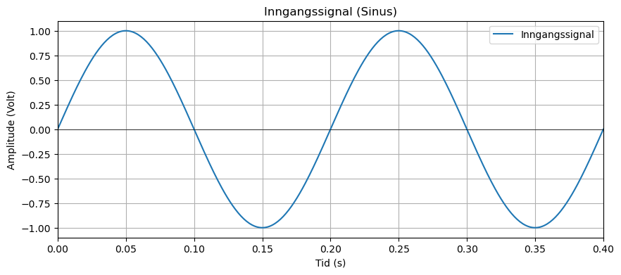
\includegraphics[width=\linewidth]{operasjonsforsterker/plot/NONInvPlot.png}
			\caption{Inngangsignal til krets}
			\label{fig:NONinvPlot}
		\end{minipage}
	\end{figure}

\end{question}

\vspace{0.5cm} % Add space after the solution

\begin{solution}[name=Løsningsforslag oppgave]


\begin{figure}[H]
	\centering
	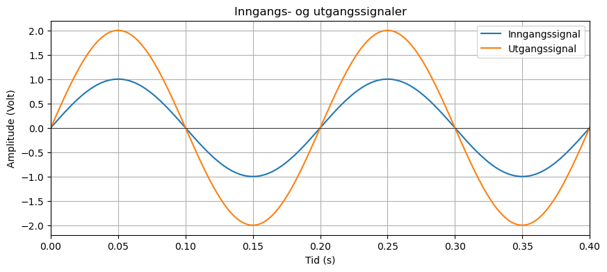
\includegraphics[width=0.7\textwidth]{operasjonsforsterker/plot/NONInvPlotSOL.png}
	\caption{Inn og utgangsignal for kretsen}
	\label{fig:NONinvPlotSol}
\end{figure}

\end{solution}
\vspace{0.5cm} % Add space after the solution

\begin{question}[name=Oppgave, topic=operasjonsforsterker]
Finn verdien for $R_2$ slik at forsterkningen blir 100.
	\begin{figure}[H]
	\centering
	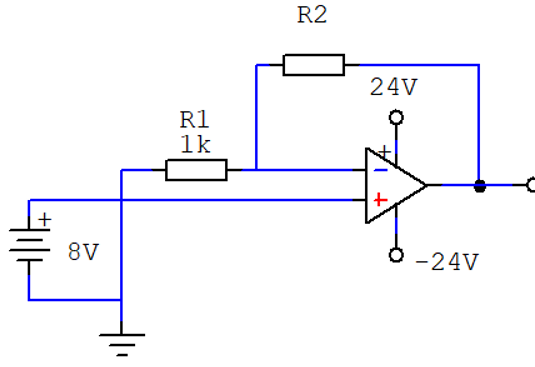
\includegraphics[width=0.6\textwidth]{operasjonsforsterker/figurer/NONinvBasic2.png}
	\caption{Operasjonsforsterkerkrets}
	\label{fig:NONinvKrets2}
\end{figure}

\end{question}

\vspace{0.5cm} % Add space after the solution

\begin{solution}[name=Løsningsforslag oppgave]
\[F_U=1+\frac{R_2}{R_1} \rightarrow 100=1+\frac{R_2}{1 \cdot 10^3} \rightarrow 100-1=\frac{R_2}{1 \cdot 10^3} \rightarrow R_2=99 \cdot 10^3=99[k\Omega] \]

\end{solution}
\vspace{0.5cm} % Add space after the solution

\begin{question}[name=Oppgave, topic=operasjonsforsterker]
Finn verdien for $U_{ut}$ i Figur \ref{fig:NONinvKrets3}.
	\begin{figure}[H]
		\centering
		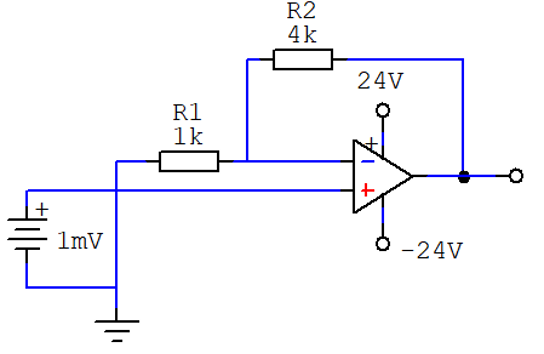
\includegraphics[width=0.6\textwidth]{operasjonsforsterker/figurer/NONinvBasic3.png}
		\caption{Operasjonsforsterkerkrets}
		\label{fig:NONinvKrets3}
	\end{figure}

\end{question}

\vspace{0.5cm} % Add space after the solution

\begin{solution}[name=Løsningsforslag oppgave]
\[U_{ut}= \left(1+\frac{R_2}{R_1}\right) \cdot U_{inn} = \left(1+\frac{4\cdot 10^3}{1 \cdot 10^3}  \right) \cdot 4 = \left(1+4 \right) \cdot 4 = 20[V]\]
\end{solution}
\vspace{0.5cm} % Add space after the solution

\begin{question}[name=Oppgave, topic=operasjonsforsterker]
Finn spenningsforsterkningen og utgangspenningen for kretsen vist i Figur \ref{fig:NONinvKrets4}.
	\begin{figure}[H]
		\centering
		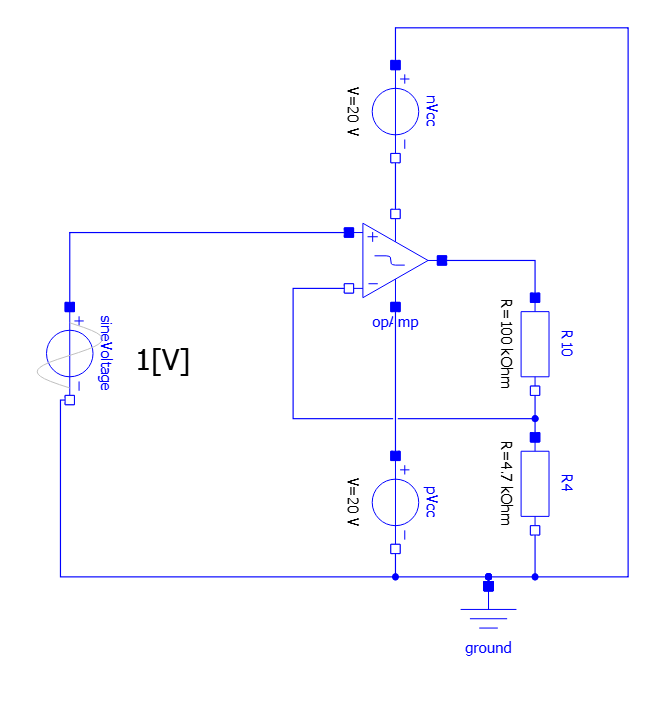
\includegraphics[width=0.6\textwidth]{operasjonsforsterker/figurer/NONinvBasic4.png}
		\caption{Operasjonsforsterkerkrets}
		\label{fig:NONinvKrets4}
	\end{figure}

\end{question}

\vspace{0.5cm} % Add space after the solution

\begin{solution}[name=Løsningsforslag oppgave]
\[F_U= 1+\frac{R_{10}}{R_4} = 1+ \frac{100\cdot10^3}{4,7\cdot10^3} = 22,3 \]

Med inngangsignal $U_{inn}=1[V]$ som merket i kretsen kan man beregne utgangspenningen.

\[U_{ut}=U_{inn} \cdot F_U= 1 \cdot 22,3 = 22,3[V]\]

Siden operasjonsforsterkeren er forsynt med $\pm 20[V]$ vil maksimal spenning på utgangen bli $20[V]$ som vist i simulering av kretsen i Figur \ref{fig:NONinvKrets4PLOT} hvor signalet holdes konstant ved $20[V]$ før utgangen faller under eller over $20[V]$ igjen.
	\begin{figure}[H]
	\centering
	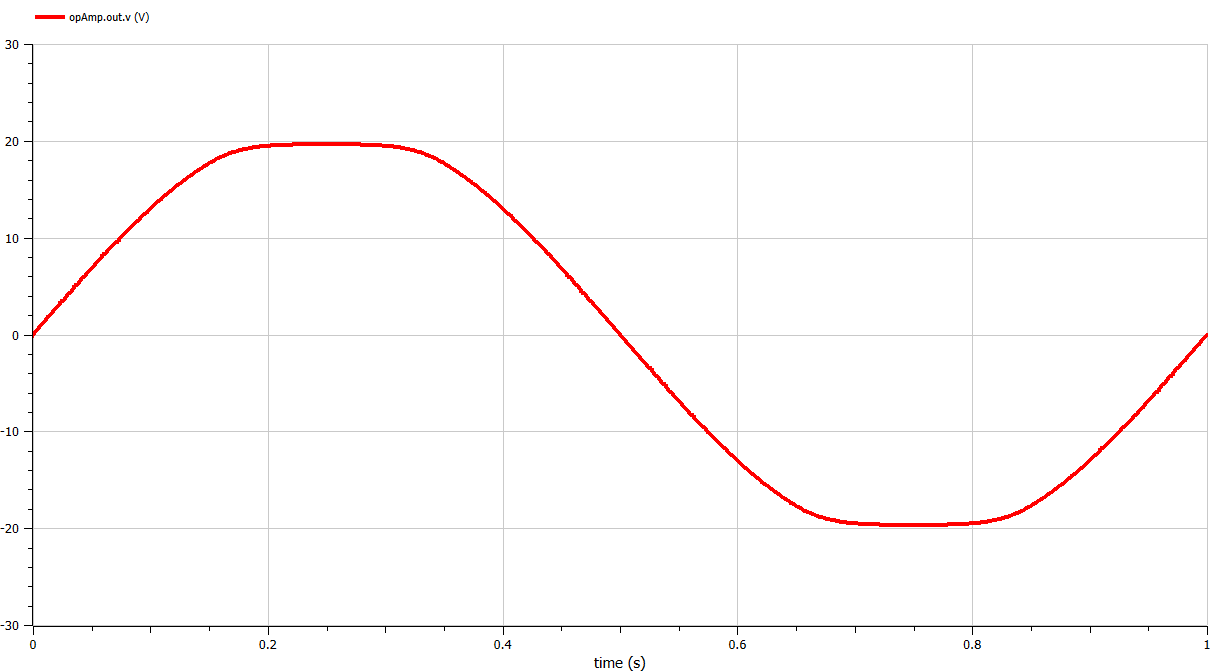
\includegraphics[width=0.6\textwidth]{operasjonsforsterker/plot/NONinvBasic4PLOT.png}
	\caption{Operasjonsforsterkerkrets - Plot}
	\label{fig:NONinvKrets4PLOT}
\end{figure}



\end{solution}
\vspace{0.5cm} % Add space after the solution




%--------------------------- SUMMERENDE KOBLING --------------------------------
\begin{question}[name=Oppgave, topic=operasjonsforsterker]
	Finn hvilken spenning måler man på utgangen av kretsen vist i \ref{fig:sumCircuit2}.

	\begin{figure}[H]
		\centering
		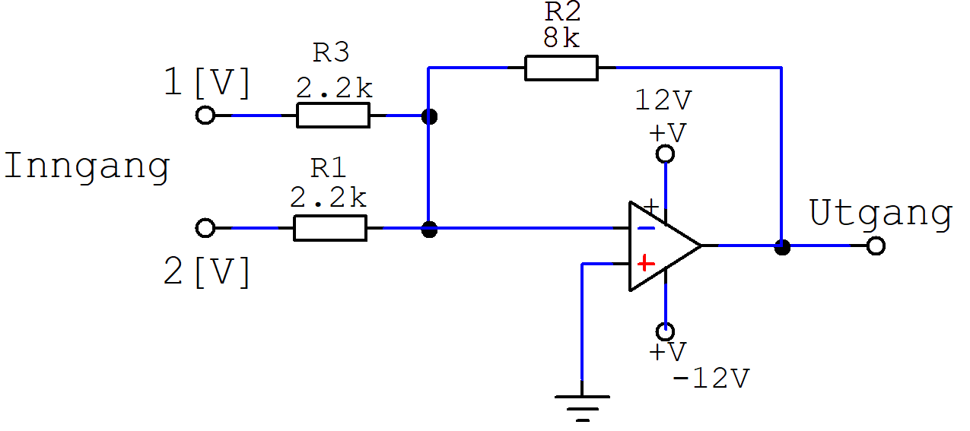
\includegraphics[width=0.8\textwidth]{operasjonsforsterker/figurer/SumKrets1.png}
		\caption{Operasjonsforsterkerkrets}
		\label{fig:sumCircuit2}
	\end{figure}

\end{question}

\vspace{0.5cm} % Add space after the solution

\begin{solution}[name=Løsningsforslag oppgave]
Løsningsalternativ 1:

Beregner de individuelle spenningsforsterkningene.
\[F_1=-\frac{R_2}{R_3}=\frac{8\cdot10^3}{2,2\cdot10^3} \approx -3,636\]
\[F_2=-\frac{R_2}{R_1}=\frac{8\cdot10^3}{2,2\cdot10^3} \approx -3,636\]

Beregner så utgangspenningen.
\[U_{ut}=F_1 \cdot U_{inn1}+F_2 \cdot U_{inn2}=3,636\cdot1+3,636\cdot2\approx 10,9[V]\]

Løsningsalternativ 2:
\[U_{ut}=- \left (\frac{U_{inn1}}{R_3}+\frac{U_{inn2}}{R_1} \right) = -\left (\frac{1}{2,2\cdot10^3}+\frac{2}{2,2\cdot10^3} \right) \cdot 8 \cdot10^3 = \frac{120}{11} \approx10,9[V]\]

\end{solution}
\vspace{0.5cm} % Add space after the solution

\begin{question}[name=Oppgave, topic=operasjonsforsterker]
Finn hvilken spenning måler man på utgangen av kretsen vist i \ref{fig:sumCircuit1}.

	\begin{figure}[H]
		\centering
		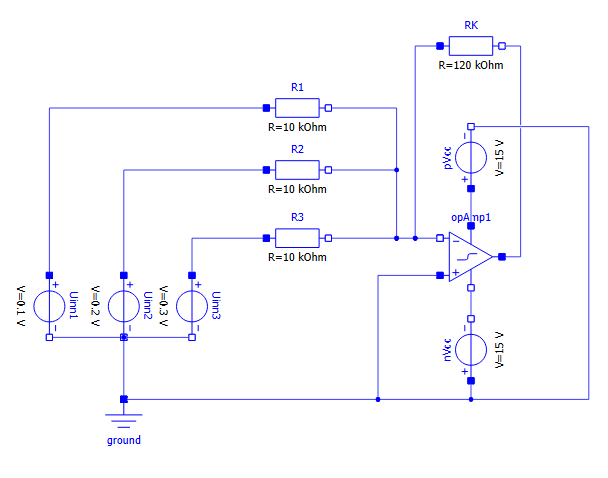
\includegraphics[width=0.8\textwidth]{operasjonsforsterker/figurer/SumKrets.png}
		\caption{Operasjonsforsterkerkrets}
		\label{fig:sumCircuit1}
	\end{figure}

\end{question}

\vspace{0.5cm} % Add space after the solution

\begin{solution}[name=Løsningsforslag oppgave]

\[U_{ut}=-\left(\frac{U_{inn1}}{R_1}+\frac{U_{inn2}}{R_2}+\frac{U_{inn3}}{R_3}\right)\cdot R_K = -\left(\frac{0,1}{10 \cdot10^3}+\frac{0,2}{10 \cdot10^3}+\frac{0,3}{10 \cdot10^3}\right)\cdot 120 \cdot 10^3 = -7,2 [V]\]

\end{solution}

\vspace{0.5cm} % Add space after the solution